\documentclass[10pt]{article}
\usepackage[a4paper,margin=0.72in]{geometry}
\usepackage{amsmath,amssymb,amsthm,mathtools}
\usepackage{graphicx}
\usepackage[hidelinks]{hyperref}
\setlength{\parindent}{0pt}
\setlength{\parskip}{0.45em}
\newtheorem{theorem}{Theorem}
\newtheorem{proposition}[theorem]{Proposition}
\newtheorem{lemma}[theorem]{Lemma}
\newcommand{\N}{\mathbb N}
\newcommand{\E}{\mathcal E}
\newcommand{\B}{\mathcal B}
\newcommand{\M}{\mathcal M}
\title{A decomposition obstruction for the Pirkovskii--Piszczek\\
$k_\infty(\N^2,V)$ example}
\author{Candidate substantial partial result for arXiv:2012.08956}
\date{11 August 2026}

\begin{document}
\maketitle

\textbf{Status.} Candidate substantial partial result, likely valid.  The
source conjecture is proved for topological \emph{algebra} isomorphisms.  For
arbitrary locally convex-space isomorphisms, a Banach-step localization and a
compact tail-corona reduction are proved; that stronger conjecture remains
open.

\section*{Source conjecture}

Pirkovskii and Piszczek \cite{PP} fix $0<c_j\leq1$ with $c_j\to0$ and define
weights on $\N^2$ by
\[
 v_n(i,j)=\begin{cases}c_j^n,&i<n,\\1,&i\geq n.\end{cases}
\]
Write
\[
 \E=k_\infty(\N^2,V)=\operatorname{ind}_n E_n,
 \qquad E_n=\ell_\infty(\N^2,v_n),
 \qquad p_n(x)=\sup_{i,j}|x_{ij}|v_n(i,j).
\]
Their Proposition 5.10(v) proves that the analogous $k_0$ space is not a
direct sum of a normed algebra and a contractible K\"othe co-echelon algebra.
They conjecture the same assertion for $\E$.

\begin{center}
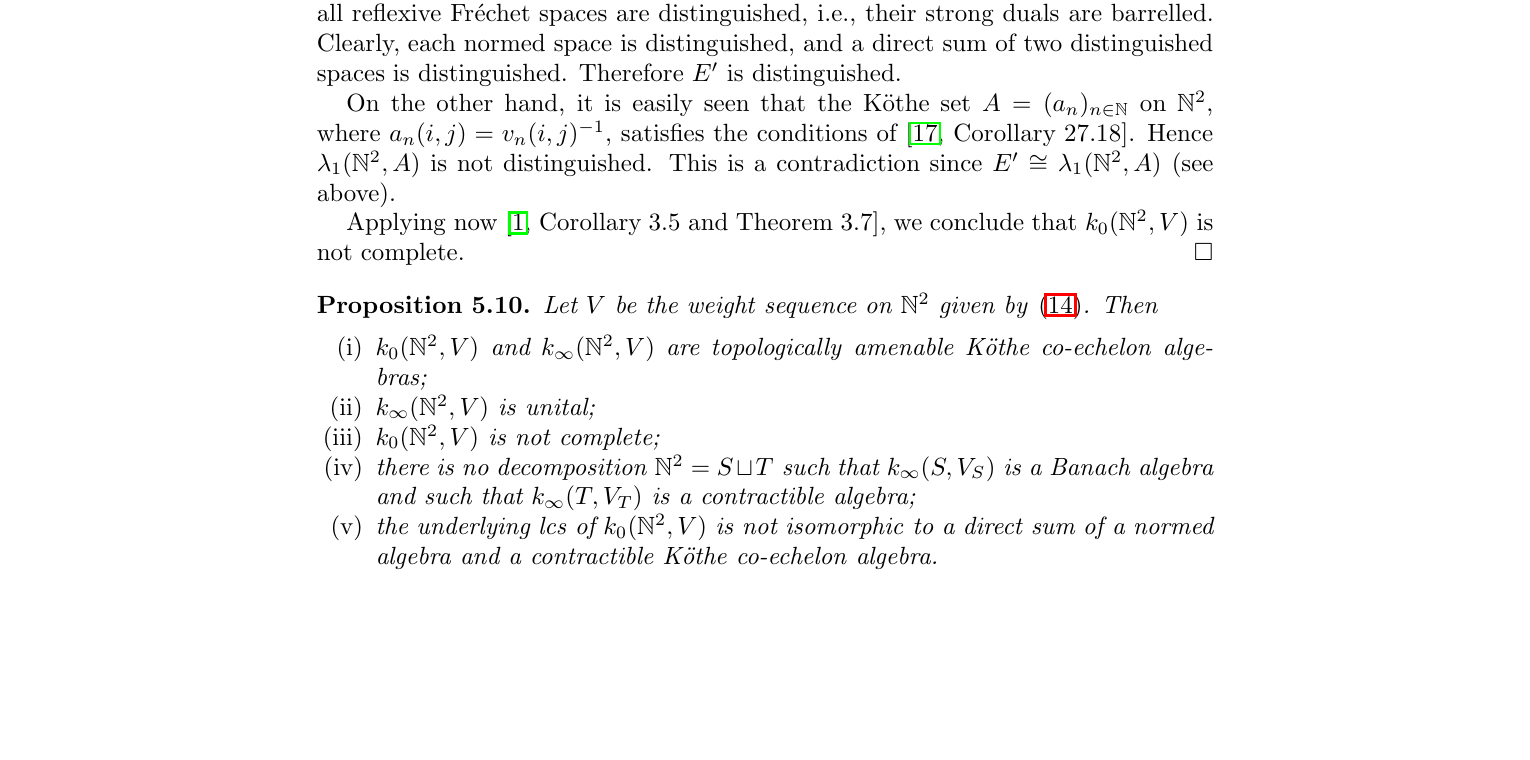
\includegraphics[width=0.97\textwidth]{figures/open_problem_context_page18.png}

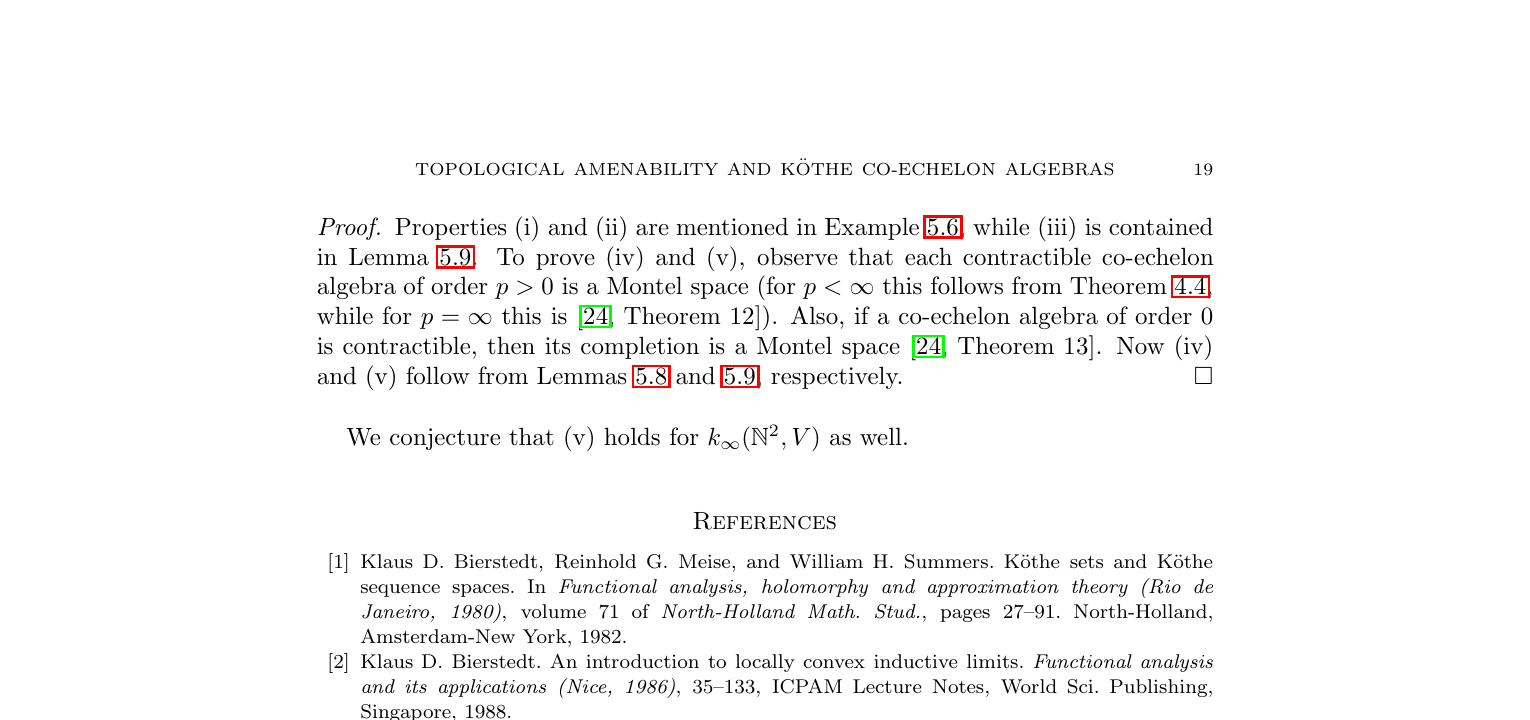
\includegraphics[width=0.97\textwidth]{figures/open_problem_conjecture_page19.png}
\end{center}

The two images are from source PDF pages 18 and 19.  The phrase ``underlying
lcs'' makes the conjecture stronger than an assertion about algebra
isomorphisms: a general linear homeomorphism need not preserve coordinate
idempotents.

\section*{Proof intuition}

For an algebra decomposition, the identity of one summand pulls back to an
idempotent of the coordinatewise algebra $\E$.  Coordinatewise idempotents are
exactly characteristic functions, so every algebra decomposition is already
one of the coordinate partitions excluded in source Lemma 5.8.

For a merely linear decomposition, replace idempotents by the continuous
projection $P$ onto the normed summand.  Baire's theorem forces its Banach
range into one fixed weighted $\ell_\infty$ step.  The complementary projection
then has Montel range, hence sends every Banach-step unit ball to a relatively
compact subset of the inductive limit.  Passing to the quotient of bounded row
arrays by row-$c_0$ arrays isolates the remaining obstruction as a compact
perturbation of the tail-corona quotient.

\section*{The algebra-isomorphism case}

\begin{theorem}\label{thm:algebra}
There is no topological algebra isomorphism
\[
             \E\cong B\oplus C
\]
where $B$ is a normed algebra and $C$ is a contractible K\"othe co-echelon
algebra.
\end{theorem}

\begin{proof}
The space $\E$ is complete \cite[Theorem 2.3]{BMS}.  The two summands are
closed complemented subspaces, so $B$ and $C$ are complete.  In particular,
$B$ is Banach.  A contractible co-echelon algebra of positive order is Montel;
for order zero its completion is Montel \cite[Theorems 12 and 13]{Piszczek}.
Thus completeness makes $C$ Montel in every case.

Let $\Phi:\E\to B\oplus C$ be the alleged algebra isomorphism.  Since $\E$ is
unital, so is $B\oplus C$, and $e=\Phi^{-1}(1_B,0)$ is an idempotent.  The
multiplication of $\E$ is coordinatewise, hence every coordinate of $e$ is
zero or one.  There is therefore a partition $\N^2=S\sqcup T$ with
$e=\mathbf 1_S$.  Multiplication by $e$ and $1-e$ gives topological
identifications
\[
 e\E=k_\infty(S,V_S),\qquad (1-e)\E=k_\infty(T,V_T).
\]
The restriction of $\Phi$ identifies the first space with the Banach space
$B$ and the second with the Montel space $C$.  This contradicts Lemma 5.8 of
\cite{PP}, which forbids exactly such a coordinate partition.
\end{proof}

\section*{Localization of any hypothetical linear decomposition}

The next lemma is useful independently of the algebra structure.

\begin{lemma}[Baire localization]\label{lem:baire}
If a Banach space $Y$ is topologically isomorphic to a linear subspace of
$\E$, then its image is contained continuously in one step $E_N$: for some
$N$ and $C<\infty$,
\[
                         p_N(y)\leq C\|y\|_Y\qquad(y\in Y).
\]
\end{lemma}

\begin{proof}
Regard each $p_n$ as an extended seminorm on $\E$, with value $+\infty$
outside $E_n$.  Its sublevel sets are closed: they are intersections of the
closed coordinate inequalities $|x_{ij}|v_n(i,j)\leq r$.  Therefore
\[
 Y=\bigcup_{n,r\in\N}\{y\in Y:p_n(y)\leq r\}
\]
is a countable union of closed sets.  By Baire's theorem, one of these sets
has nonempty interior.  Taking differences gives a neighborhood of zero on
which $p_N$ is bounded.  Homogeneity then yields the displayed estimate on
all of $Y$.
\end{proof}

\begin{proposition}[compact-projection reduction]\label{prop:projection}
Suppose, as locally convex spaces, that
\[
                         \E=B_0\oplus M_0,
\]
where $B_0$ is normed and $M_0$ is a contractible K\"othe co-echelon algebra.
Let $P$ and $Q=I-P$ be the associated projections.  Then:
\begin{enumerate}
\item $B_0$ is Banach and $M_0$ is Montel;
\item for some $N$, $B_0\subset E_N$ continuously;
\item $B_0$ is complemented in every $E_m$ for $m\geq N$;
\item for every $m\geq N$, $Q|_{E_m}:E_m\to\E$ is compact in the locally
convex sense.
\end{enumerate}
\end{proposition}

\begin{proof}
The first assertion follows exactly as in the first paragraph of
Theorem~\ref{thm:algebra}.  Lemma~\ref{lem:baire} gives (2).  For $m\geq N$,
$P|_{E_m}$ is a bounded map into the Banach space $B_0$ and is the identity on
$B_0$, proving (3).  Finally, the unit ball of $E_m$ is bounded in $\E$; its
$Q$-image is bounded in the Montel space $M_0$, hence relatively compact in
$M_0$ and therefore in $\E$.
\end{proof}

\section*{Tail-corona form of the remaining obstruction}

Put
\[
 X=\ell_\infty(\N;\ell_\infty(\N)),\qquad
 X_0=c_0(\N;\ell_\infty(\N)),\qquad Z=X/X_0,
\]
and let $q:X\to Z$ be the quotient map.  We identify $X$ with $E_1$.

\begin{proposition}[tail-corona factorization]\label{prop:corona}
There is a continuous linear map $\Pi:\E\to Z$ whose restriction to $E_1=X$
is $q$.  Under the hypotheses of Proposition~\ref{prop:projection}, let
$B_0\subset E_N$ and let $R_N:B_0\to X$ delete the first $N-1$ rows.  Then
\[
                  q=qR_NP|_X+K,
                  \qquad K:X\to Z\ \hbox{compact}.
\]
\end{proposition}

\begin{proof}
For $x\in E_n$, delete the first $n-1$ rows.  The remaining array is bounded,
with $X$-norm at most $p_n(x)$.  If a later step is used, the two bounded
representatives differ in finitely many rows and hence by an element of $X_0$.
This defines $\Pi$ unambiguously.  Its restriction to each $E_n$ is bounded,
so the inductive-limit property makes $\Pi$ continuous; on $E_1$ it is $q$.

For $b\in B_0\subset E_N$, tail deletion gives
$\Pi(b)=qR_N(b)$.  On $X$ we have
\[
 q=\Pi(P+Q)|_X=qR_NP|_X+\Pi Q|_X.
\]
By Proposition~\ref{prop:projection}, $Q|_X$ maps the unit ball to a relatively
compact subset of $\E$.  Its composition $K=\Pi Q|_X$ is therefore compact.
\end{proof}

\section*{Scope, verification, and novelty}

Theorem~\ref{thm:algebra} strictly extends source Proposition 5.10(iv) from
coordinate partitions to all topological algebra decompositions.  It does not
settle the source wording, which concerns arbitrary locally convex-space
isomorphisms.  Propositions~\ref{prop:projection} and \ref{prop:corona} give a
necessary condition for such an isomorphism.

A tempting final step would use the moving-row copy of $c_0$ and the fact that
$B_0$ is complemented in a Banach space isomorphic to $\ell_\infty$.  The gap
is that $Q|_{E_N}$ is compact only into the inductive-limit topology, not
necessarily in the fixed $E_N$ norm.  No claim requiring that invalid upgrade
is made.

The idempotent computation, every closed-set step in Lemma~\ref{lem:baire},
and independence of the tail representative were checked directly.  No
computation is used.  A bounded novelty search on 11 August 2026 covered the
run indexes and exact-phrase/keyword web searches for the conjecture and its
decomposition terms.  The source and published version were found, but no
later resolution.  Novelty confidence is moderate because the ingredients are
standard, while this application was not located.

\textbf{Human-review recommendation.} Check first the order-zero completeness
point and Lemma~\ref{lem:baire}.  For an upgrade, test whether the factorization
in Proposition~\ref{prop:corona} is incompatible with a projection extending
continuously to every weighted step; do not replace inductive-limit compactness
by fixed-step norm compactness.

\begin{thebibliography}{9}
\bibitem{PP}
A. Yu. Pirkovskii and K. Piszczek,
\emph{Topological amenability and K\"othe co-echelon algebras},
Banach J. Math. Anal. 16 (2022), Article 13; arXiv:2012.08956.

\bibitem{BMS}
K. D. Bierstedt, R. G. Meise, and W. H. Summers,
\emph{K\"othe sets and K\"othe sequence spaces},
North-Holland Math. Stud. 71 (1982), 27--91.

\bibitem{Piszczek}
K. Piszczek,
\emph{Contractible K\"othe co-echelon algebras},
Quaest. Math. 43 (2020), 493--505.
\end{thebibliography}

\end{document}

